\chapter{Theoretische Grundlagen}

Um die Funktionsweise von Augmented Reality und verwandten Technologien zu verstehen, ist ein grundlegendes Wissen über die zugrunde liegenden Konzepte und Technologien erforderlich. In diesem Kapitel werden die theoretischen Grundlagen der AR erläutert, die für die Entwicklung von mobilen Anwendungen relevant sind. Dazu gehören Themen, wie die Sensorik, die Kalibrierung, das Tracking und die dreidimensionale Rekonstruktion der Umgebung. \cite{doerner2022virtual}

\section{Mathematische und Geometrische Grundlagen}

Die Mathematik bildet die Grundlage für viele Algorithmen und Technologien in der Augmented Reality. Insbesondere die Geometrie und Algebra spielen eine wichtige Rolle bei der Bestimmung der Position und Orientierung von Objekten in der realen Welt. In diesem Abschnitt werden die mathematischen Grundlagen erläutert, die für die Entwicklung von AR-Anwendungen relevant sind.

\subsection{Dreidimensionale Computergrafik}

In der Computergrafik werden dreidimensionale Objekte, auch als Modelle bezeichnet, durch geometrische und relationale Informationen beschrieben. Diese Objekte bestehen in der Regel aus Polygonen, die durch ihre Eckpunkte (\emph{Vertices}) definiert sind. Ein Polygon ist eine geschlossene Fläche (\emph{Face}), die durch das Verbinden der Vertices mit geraden Linien entsteht. \cite{wikipedia2023polygons, espinoza2024graphics}

Die einfachsten Polygone sind Dreiecke, die die Grundbausteine der Computergrafik und die Basis für die Darstellung komplexerer Objekte bilden. Obwohl komplexere Polygone existieren, werden diese oft in Dreiecke zerlegt, da diese von Grafik-Pipelines effizienter verarbeitet werden können. Solche Modelle bestehen dann aus Dreiecksnetzen (\emph{Meshes}), die als Arrays von Vertices und Indizes gespeichert werden. \cite{wikipedia2023polygons, espinoza2024graphics}

Abbildung \ref{fig:TriangleMesh} zeigt das Polygonnetz eines Delfins. Um dieses Modell im dreidimensionalen Raum zu transformieren, werden mathematische Konzepte wie Vektoren, Matrizen und Transformationen verwendet. Diese Konzepte bilden die Grundlage für die Positionierung und Darstellung von 3D-Objekten in der Augmented Reality und werden in den kommenden Abschnitten näher erläutert. \cite{wikipedia2023mesh, espinoza2024graphics}

\begin{figure}
    \centering
    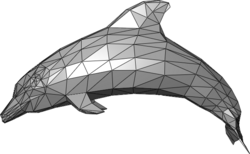
\includegraphics[ width=.5\textwidth ]{TriangleMesh}
    \caption{Dreiecksnetz eines Delfin-Modells \cite{wikipedia2023mesh}\label{fig:TriangleMesh}}\par
\end{figure}

\subsection{Koordinationssysteme}

Dreidimensionale Szenen und Objekte werden in kartesischen Koordinatensystemen beschrieben. Man unterscheidet zwischen verschiedenen Koordinatensystemen, die für unterschiedliche Zwecke verwendet werden. Gängige Koordinatensysteme in der Computergrafik sind das Weltkoordinatensystem, das Kamerakoordinatensystem und das Objektkoordinatensystem. Während das Weltkoordinatensystem als festes Referenzkoordinatensystem dient und die Position sowie Orientierung von Objekten im Raum definiert, beschreibt das Objektkoordinatensystem die Position der Vertices eines Objekts relativ zu dessen eigenem Ursprung. \cite{doerner2022virtual, gao2021vSLAM, usau2023appleARCamera}

Die Koordinatensysteme weisen \(x\)-, \(y\)- und \(z\)-Achsen auf, die die drei Dimensionen repräsentieren. In einem rechtshändigen Koordinatensystem zeigt die \(x\)-Achse nach rechts, die \(y\)-Achse nach oben und die \(z\)-Achse entgegengesetzt der Blickrichtung (siehe Abbildung \ref{fig:Koordinatensystem}). Die Vertices eines dreidimensionalen Objekts werden durch die Koordinaten \(x\), \(y\) und \(z\) definiert. Diese Koordinaten werden meist als Vektoren dargestellt, die die Position eines Punktes im Raum beschreiben. Ein Vektor \(v\) wird durch die Koordinaten \(x\), \(y\) und \(z\) wie folgt definiert (\cite{doerner2022virtual, gao2021vSLAM, freescale2010math3d, pezzi2021matrices}):

\begin{equation}
v = \begin{bmatrix} x \\ y \\ z \end{bmatrix}
\end{equation}

\begin{figure}
    \centering
    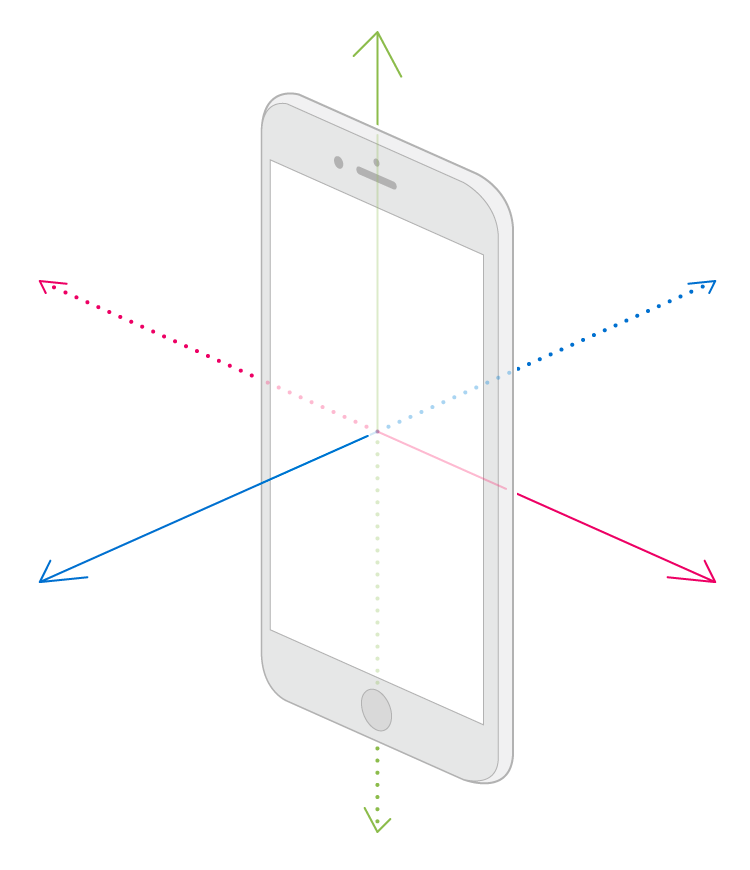
\includegraphics[ width=.5\textwidth ]{CoordinateSystem}
    \caption{Rechtshändiges Koordinatensystem \cite{appledevdoc}\label{fig:Koordinatensystem}}\par
\end{figure}

\subsection{Transformationsmatrizen}

Eine Transformation beschreibt die Änderung der Position, Orientierung oder Skalierung eines Objekts im Raum. In der Computergrafik werden Transformationen mithilfe von Matrizen durchgeführt, die die Koordinaten eines Objekts in ein anderes Koordinatensystem überführen. Die wichtigsten Transformationen sind Translation, Rotation und Skalierung, die durch spezielle Transformationsmatrizen beschrieben werden. \cite{doerner2022virtual, gao2021vSLAM, pezzi2021matrices}

Um die Translation und Rotation mit einer einzigen Transformationsmatrix zu beschreiben, werden homogene Koordinaten verwendet. Homogene Koordinaten erweitern den dreidimensionalen Vektor um eine vierte Dimension, die als W-Koordinate bezeichnet wird. Die homogenen Koordinaten eines Punktes \(P\) werden als Vektor \(P_h\) dargestellt (\cite{doerner2022virtual, gao2021vSLAM, freescale2010math3d}):

\begin{equation}
P_h = \begin{bmatrix} x \\ y \\ z \\ 1 \end{bmatrix}
\end{equation}

Diese Erweiterung ermöglicht die Darstellung von Translationen als Matrixmultiplikation. Die Transformationsmatrix, die die Translation /( t /) und die Rotation /( R /) kombiniert, wird wie folgt definiert \cite{doerner2022virtual, gao2021vSLAM, freescale2010math3d}:

\begin{equation}
T = \begin{bmatrix} R & t \\ 0^T & 1 \end{bmatrix} = 
\begin{bmatrix} 
    r_{11} & r_{12} & r_{13} & t_x \\ 
    r_{21} & r_{22} & r_{23} & t_y \\ 
    r_{31} & r_{32} & r_{33} & t_z \\ 
    0 & 0 & 0 & 1 
\end{bmatrix}
\end{equation}

Hierbei entspricht /( R /) der Rotationsmatrix und /( t /) dem Translationsvektor. Die Transformationsmatrix /( T /) wird auf den homogenen Vektor \(P_h\) angewendet, um die transformierten Koordinaten \(P'_h\) zu erhalten \cite{doerner2022virtual, gao2021vSLAM, freescale2010math3d}:

\begin{equation} 
    P'_h = T \cdot P_h \label{eq:transformationsmatrix}
\end{equation}

In diesem Zusammenhang wird die Rotation oft durch eine \(3\times3\) Rotationsmatrix /( R /) beschrieben, die die Drehung um die \(x\)-, \(y\)- und \(z\)-Achsen repräsentiert. Die Rotationen um die drei Achsen werden durch die Matrizen \(R_x\), \(R_y\) und \(R_z\) beschrieben \cite{doerner2022virtual, gao2021vSLAM, freescale2010math3d}:


\begin{equation}
    R_x(\alpha) =
    \begin{bmatrix}
        1 & 0 & 0 & 0 \\
        0 & \cos(\alpha) & -\sin(\alpha) & 0 \\
        0 & \sin(\alpha) & \cos(\alpha) & 0 \\
        0 & 0 & 0 & 1
    \end{bmatrix}
\end{equation}

\begin{equation}
    R_y(\alpha) =
    \begin{bmatrix}
        \cos(\alpha) & 0 & \sin(\alpha) & 0 \\
        0 & 1 & 0 & 0 \\
        -\sin(\alpha) & 0 & \cos(\alpha) & 0 \\
        0 & 0 & 0 & 1
    \end{bmatrix}
\end{equation}

\begin{equation}
    R_z(\alpha) =
    \begin{bmatrix}
        \cos(\alpha) & -\sin(\alpha) & 0 & 0 \\
        \sin(\alpha) & \cos(\alpha) & 0 & 0 \\
        0 & 0 & 1 & 0 \\
        0 & 0 & 0 & 1
    \end{bmatrix}
\end{equation}

Zusätzlich zu den Transformationen Translation und Rotation können auch Skalierungen durchgeführt werden. Die Skalierungsmatrix S wird wie folgt definiert \cite{doerner2022virtual, gao2021vSLAM, freescale2010math3d}:

\begin{equation}
    S = 
    \begin{bmatrix} 
        s_x & 0 & 0 & 0 \\ 
        0 & s_y & 0 & 0 \\ 
        0 & 0 & s_z & 0 \\ 
        0 & 0 & 0 & 1 
    \end{bmatrix}
\end{equation}

Die Transformationsmatrix wird, wie eingehend erläutert, häufig verwendet, um dreidimensionale Modelle vom lokalen Koordinatensystem in das Weltkoordinatensystem zu überführen. Entsprechend der Gleichung \ref{eq:transformationsmatrix}, werden dazu die lokalen Koordinaten \( P_{\text{local}} \) der Vertices des 3D-Modells mit der Transformationsmatrix \( T_{\text{world}} \) multipliziert, um die Weltkoordinaten \( P_{\text{world}} \) zu erhalten \cite{doerner2022virtual, gao2021vSLAM, freescale2010math3d}:

\begin{equation}
    P_{\text{world}} = T_{\text{world}} \cdot P_{\text{local}}
\end{equation}

\section{Sensorik}

Die Umgebung wird in Augmented-Reality-Anwendungen mithilfe verschiedener Sensoren erfasst, die Daten über die physische Welt liefern. Je nach Anwendungsfall und Eingabegerät können unterschiedliche Sensoren verwendet werden, um die Position und Bewegung des Geräts zu bestimmen. Bei vielen Tracking-Verfahren werden eine Kombination von Sensoren verwendet, um die Genauigkeit und Zuverlässigkeit der Positionsschätzung zu verbessern. Beispielsweise kann die Kamera für visuelle Tracking-Anwendungen verwendet werden, während inertiale Sensoren primär für die Schätzung der Bewegung des Geräts verwendet wird. Durch die Fusion von Daten aus verschiedenen Sensoren können AR-Anwendungen eine präzise und konsistente Darstellung der virtuellen Objekte in der realen Welt erreichen. Die wichtigsten Sensorenarten für die Implementierung von AR-Anwendungen für mobile Smartgeräte werden in diesem Abschnitt erläutert. \cite{doerner2022virtual}

\subsection{Inertiale Sensoren}

Inertiale Sensoren erfassen die Bewegung und Ausrichtung eines Geräts, indem sie Beschleunigung und Rotation messen. Sie bestehen typischerweise aus zwei Hauptkomponenten: einem Gyroskop und einem Beschleunigungsmesser. Das Gyroskop misst die Winkelgeschwindigkeit und erkennt Drehbewegungen, während der Beschleunigungsmesser lineare Beschleunigungen erfasst. Durch die Kombination beider Sensoren in einer Inertial Measurement Unit (IMU) können Bewegungen in sechs Freiheitsgraden (dreidimensionale Position und Orientierung) bestimmt werden. Diese Technologie ist essenziell für die Echtzeiterfassung von Bewegungen und wird in AR-Brillen, Smartphones sowie anderen mobilen Geräten eingesetzt. \cite{doerner2022virtual}

\begin{tcolorbox}[colback=THAi-Blue!20!white, colframe=THAi-Blue]
    Als \textbf{Freiheitsgrade} (engl. Degrees of Freedom – DOF) werden voneinander unabhängige Bewegungsmöglichkeiten eines physikalischen Systems bezeichnet. Ein starrer Körper besitzt sechs Freiheitsgrade: je drei für die Translation und Rotation. \cite{wikipedia2024dof}
\end{tcolorbox}  

\subsection{Kamera}

Die Kamera spielt eine zentrale Rolle in AR-Anwendungen, da sie visuelle Informationen erfasst, die für viele Tracking-Verfahren essenziell sind. Die aufgenommenen Bilder dienen nicht nur als Grundlage der Ausgabe für die Darstellung virtueller Objekte, sondern ermöglichen auch die Erkennung von Markern, Merkmalen oder Objekten. Durch die Analyse dieser Bilddaten kann die Position und Orientierung des Geräts bestimmt werden, wodurch eine präzise Überlagerung virtueller Inhalte mit der realen Umgebung ermöglicht wird. \cite{doerner2022virtual}

\subsection{Lasersensoren}\label{LiDAR}

LiDAR-Sensoren (\emph{Light Detection and Ranging}) sind eine spezielle Art von Lasersensoren, die die Entfernung zu Objekten mithilfe von Laserstrahlen messen. Dabei wird, entsprechend des ToF-Prinzips (\emph{Time of Flight}), die Zeit gemessen, die das Licht benötigt, um von der Lichtquelle zum Objekt und zurück zum Sensor zu gelangen. Durch die Messung der Laufzeit des Lichts kann die Entfernung zum Objekt präzise bestimmt werden. LiDAR-Sensoren sind besonders nützlich für die Erfassung von Tiefeninformationen in der Umgebung und bieten große Vorteile für die Genauigkeit und Zuverlässigkeit des Trackings in AR-Anwendungen. \cite{doerner2022virtual, ibm2024lidar}

\subsection{Magnetfeldbasierte Sensoren}

Magnetfeldbasierte Sensoren, wie das Magnetometer in \emph{Inertial Measurement Units} (IMU), messen das Erdmagnetfeld und ermöglichen so die Bestimmung der Geräteausrichtung relativ zu den magnetischen Feldlinien. Sie spielen eine wichtige Rolle bei der Orientierung im Raum und ergänzen andere Sensoren zur präzisen Positionsbestimmung in AR-Anwendungen. \cite{doerner2022virtual}

Allerdings sind Magnetometer anfällig für Störungen durch elektrische Geräte, Metallgegenstände und magnetische Felder in der Umgebung, was die Genauigkeit der Messungen beeinträchtigen kann. Trotz dieser Einschränkungen sind sie eine wertvolle Ergänzung zu Gyroskopen und Beschleunigungssensoren, da sie zur Stabilisierung und Korrektur der Ausrichtung beitragen. \cite{doerner2022virtual}

\section{Kalibrierung}\label{Kalibrierung}

Die Kalibrierung ist ein zentraler Schritt in der Augmented-Reality-Pipeline, da sie die Bestimmung der intrinsischen und extrinsischen Kameraparameter ermöglicht. Diese Parameter sind essenziell, um Bildpunkte korrekt in die dreidimensionalen Weltkoordinaten zu transformieren. \cite{mw2024calibration}

Ein häufig verwendetes Modell zur Beschreibung der Kamera ist das \emph{Pinhole}-Kameramodell, das die grundlegenden Eigenschaften einer idealisierten Kamera abstrahiert (siehe Abbildung \ref{fig:Pinhole}). Es geht von einer Kamera ohne Objektiv aus, die lediglich eine kleine Blendenöffnung besitzt. Das Licht tritt durch diese Öffnung ein und projiziert ein invertiertes Abbild der Szene auf eine Bildebene. \cite{mw2024calibration}

Durch die Kalibrierung lassen sich die intrinsischen und extrinsischen Parameter bestimmen, die gemeinsam eine Projektionsmatrix definieren. Diese Matrix ermöglicht die Umrechnung von Bildkoordinaten in das reale 3D-Koordinatensystem (siehe Abbildung \ref{fig:Kalibrierung}). Die intrinsischen Parameter umfassen die Brennweite, die Objektivverzerrung und die Position des optischen Zentrums der Kamera. Die extrinsischen Parameter hingegen beschreiben die Position und Orientierung der Kamera im Raum. \cite{mw2024calibration}

\begin{figure}[h]
    \centering
    \begin{minipage}{0.45\textwidth}
        \centering
        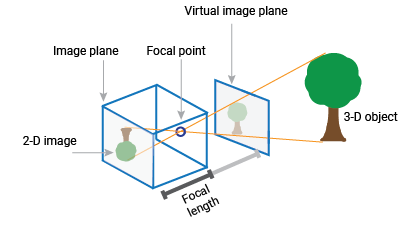
\includegraphics[width=\textwidth]{pinhole}
        \caption{Pinhole-Modell \cite{mw2024calibration}\label{fig:Pinhole}}
    \end{minipage}
    \hfill
    \begin{minipage}{0.45\textwidth}
        \centering
        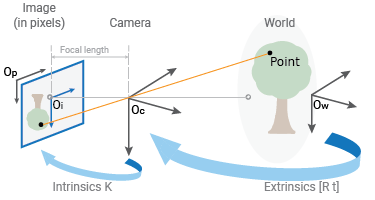
\includegraphics[width=\textwidth]{calibration-cameramodel-coords}
        \caption{Modell für die Kamerakalibrierung \cite{mw2024calibration}\label{fig:Kalibrierung}}
    \end{minipage}
\end{figure}

Es gibt verschiedene Methoden zur Kamerakalibrierung, die auf unterschiedlichen Ansätzen basieren. Eine der bekanntesten Methoden ist die \emph{Flexible camera calibration by viewing a plane from unknown orientations} \cite{zhang1999calibration}, die auf der Verwendung eines Schachbrettmusters mit bekannten Dimensionen beruht. Dabei wird das Schachbrettmuster aus verschiedenen Perspektiven aufgenommen, um die intrinsischen und extrinsischen Parameter der Kamera zu bestimmen. \cite{stachniss2021calibration, zhang1999calibration}

\subsection{Mathematische Beschreibung der Projektionsmatrix}

Mathematisch wird die Projektionsmatrix \(P\) wie folgt definiert \cite{mw2024calibration, szeliski2022computerVision}:

\[
P = K[R|t]
\]

Hierbei entspricht \(K\) der intrinsischen Matrix, \(R\) die Rotationsmatrix und \(t\) der Translationsvektor der extrinsischen Matrix. Die intrinsische Matrix \(K\) ist definiert als \cite{mw2024calibration}:

\[
K = 
\begin{bmatrix}
f_x & s & c_x \\
0 & f_y & c_y \\
0 & 0 & 1
\end{bmatrix}
\]

Dabei gilt:

\begin{itemize}
    \item \( f_x \) und \( f_y \): Brennweiten der Kamera in Pixeln, bezogen auf die horizontalen und vertikalen Achsen.
    \item \( c_x \) und \( c_y \): Koordinaten des optischen Zentrums in Pixeln.
    \item \( s \): Skew-Faktor, der berücksichtigt, ob die Kameraachsen orthogonal sind.
\end{itemize}

Ein Punkt im dreidimensionalen Raum \( X = [X, Y, Z, 1]^T \) wird mithilfe der folgenden Gleichung in das Bildkoordinatensystem \( x = [x, y, 1]^T \) projiziert \cite{mw2024calibration}:

\[
x = PX
\]

\subsection{Objektivverzerrungen und Korrektur}

Ein wichtiger Bestandteil der Kalibrierung ist die Korrektur von Objektivverzerrungen, da sie die Genauigkeit der Projektion beeinträchtigen können. Diese Verzerrungen entstehen durch die Krümmung der Linse (radiale Verzerrung, siehe Abbildung \ref{fig:Distortion}) oder durch Fehlausrichtungen zwischen Linse und Sensor (tangentiale Verzerrung). Werden sie nicht berücksichtigt, können sich Fehler in der Umrechnung zwischen Bild- und Weltkoordinaten ergeben. \cite{mw2024calibration, szeliski2022computerVision}

\begin{figure}[h]
    \centering
    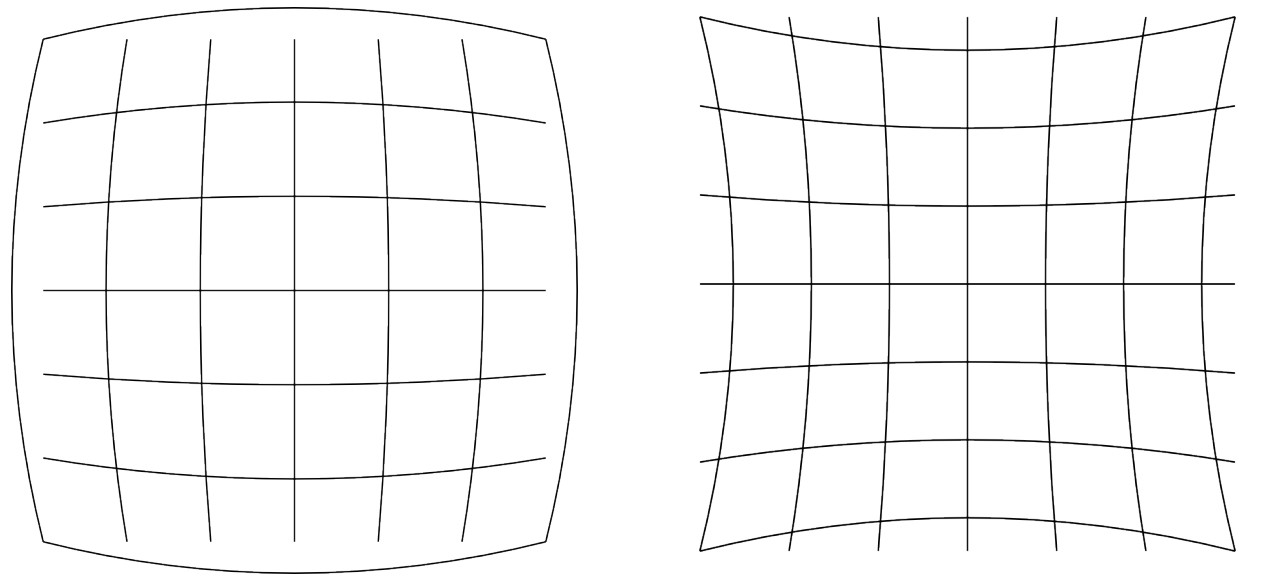
\includegraphics[width=.5\textwidth]{Distortion}
    \caption{Radiale Verzerrungen der Linse \cite{stachniss2021calibration}\label{fig:Distortion}}
\end{figure}

Dazu werden oft Polynommodelle, wie das \emph{Brown-Conrady-Modell}, verwendet. Dieses Modell beschreibt die relative Position eines Punktes zwischen der Linse und des Sensors. Die radiale und tangentiale Verzerrung der Linse wird durch die Koeffizienten \( k_1, k_2, k_3 \) und \( p_1, p_2 \) bestimmt \cite{brown1966distortion} und wie folgt beschrieben \cite{mw2024calibration, szeliski2022computerVision}:
\begin{itemize}
    \item \textbf{Radiale Verzerrung}:
    \[ x_{\text{corr}} = x \left( 1 + k_1 r^2 + k_2 r^4 + k_3 r^6 \right) \]
    \[ y_{\text{corr}} = y \left( 1 + k_1 r^2 + k_2 r^4 + k_3 r^6 \right) \]
    \item \textbf{Tangentiale Verzerrung}:
    \[ x_{\text{corr}} = x + [2p_1xy + p_2(r^2 + 2x^2)] \]
    \[ y_{\text{corr}} = y + [p_1(r^2 + 2y^2) + 2p_2xy] \]
\end{itemize}

\subsection{Praktische Relevanz der Kalibrierung in AR}

In den vorangegangenen Abschnitten wurde die Kamerakalibrierung anhand einfacher Modelle erläutert. In der Praxis sind die intrinsischen Parameter jedoch bereits vorkalibriert und können von den Herstellern der Kameras bereitgestellt werden. So integriert zum Beispiel Apples Augmented-Reality-Framework (ARKit) die intrinsischen Kameraparameter und stellt sie über die Klasse \texttt{AVCameraCalibrationData} zur Verfügung. \cite{appledevdoc}

Die extrinsischen Parameter hingegen müssen häufig manuell bestimmt werden, um die exakte Position und Orientierung des Geräts im dreidimensionalen Raum zu ermitteln. In der Augmented Reality ist die präzise Bestimmung der Kameraposition essenziell für viele Tracking-Verfahren. Dabei unterscheidet man zwischen markerbasiertem Tracking, bei dem die extrinsischen Parameter mithilfe eines Markers mit bekannten Dimensionen in der Umgebung bestimmt werden, und markerlosem Tracking, bei dem die Bewegung der Kamera anhand von Merkmalen in den Bilddaten bestimmt wird. Im Kontext mobiler AR-Anwendungen sind markerlose Tracking-Verfahren, wie SLAM (siehe Kapitel \ref{SLAM}), aufgrund ihrer Flexibilität besonders relevant. Deswegen wird der Fokus in den folgenden Abschnitten auf diese Verfahren gelegt. \cite{doerner2022virtual, alam2024calibration}

\begin{tcolorbox}[colback=THAi-Blue!20!white, colframe=THAi-Blue]
    \textbf{Tracking} bezeichnet die räumliche Verfolgung von bewegten Objekten in Echtzeit oder nachträglich anhand von Aufzeichnungen. Es dient der Erfassung und Modellierung von Bewegungen, beispielsweise zur Positionsbestimmung oder zur Synchronisation mit anderen Objekten. \cite{wikipedia2024tracking}
\end{tcolorbox}  

\section{Simultaneous Localization and Mapping}\label{SLAM}

Markerloses Tracking spielt eine entscheidende Rolle in mobilen AR-Anwendungen, da es keine speziellen Markierungen in der Umgebung erfordert, um die Position und Orientierung des Geräts zu bestimmen. Dadurch können AR-Anwendungen flexibel und in beliebigen Umgebungen eingesetzt werden, was ihre Vielseitigkeit erheblich steigert. \cite{doerner2022virtual}

Neben dem Tracking ist auch die Rekonstruktion der Umgebung ein essenzieller Bestandteil der Augmented Reality. Die dreidimensionale Erfassung der Umgebung ermöglicht die realitätsnahe Platzierung virtueller Objekte, wodurch eine immersive Nutzererfahrung entsteht. \cite{doerner2022virtual}

In den letzten Jahrzehnten wurden verschiedene Verfahren entwickelt, um die Position und Orientierung eines Geräts zu bestimmen und die Umgebung dreidimensional zu rekonstruieren. Eines der bekanntesten Verfahren ist das \emph{Structure from Motion}-Verfahren (SfM), das die 3D-Struktur einer Szene anhand einer Sequenz von 2D-Bildern rekonstruiert. SfM bildet die Grundlage für viele Tracking-Methoden in der Augmented Reality, insbesondere für \emph{Simultaneous Localization and Mapping} (SLAM). \cite{doerner2022virtual, tourani2022vSLAMTrends}

Als Verfahren der zwei größten Augmented-Reality-Plattformen, ARKit von Apple und ARCore von Google, hat sich SLAM als eines der wichtigsten Technologien in der Augmented Reality etabliert. Das Verfahren, das ursprünglich aus der Robotik stammt, stellt eine effiziente und zuverlässige Möglichkeit für die \textbf{gleichzeitige} Positionsbestimmung  eines Geräts und die Extraktion dreidimensionaler Informationen der Umgebung dar. \cite{appledevdoc,arcoredevdoc, doerner2022virtual}

Es existieren verschiedene SLAM-Varianten, die sich in der Art der Sensoren, der Umgebung und der Anwendung unterscheiden. In mobilen AR-Anwendungen werden häufig visuelle SLAM-Verfahren eingesetzt, die auf Bilddaten von Kamerasensoren basieren. \cite{tourani2022vSLAMTrends}

Abbildung \ref{fig:VSLAM} zeigt die wichtigsten Schritte des vSLAM-Algorithmus. Das Verfahren besteht aus zwei Hauptkomponenten: dem \emph{Tracking} (Frontend) und dem \emph{Mapping} bzw. der \emph{Loop Detection/Closure} (Backend). Das Tracking umfasst die Schätzung der Kameraposition mithilfe der Nachverfolgung von Merkmalspunkten in den Bilddaten. Das Mapping hingegen beinhaltet die Rekonstruktion der Umgebung, indem die Positionen der Merkmale im dreidimensionalen Raum bestimmt werden. Die Loop Closure Detection dient dazu, bereits besuchte Orte in der Umgebung zu erkennen und die Konsistenz der Karte zu gewährleisten. Zusätzlich berücksichtigt SLAM eine Reihe von Optimierungsverfahren, wie das Bundle Adjustment, um die Genauigkeit der Schätzungen zu verbessern. \cite{gao2021vSLAM, tourani2022vSLAMTrends}

Im Folgenden wird der Fokus zunächst auf das Visual SLAM gelegt, da es in mobilen AR-Anwendungen weit verbreitet ist und eine ausführliche Erklärung aller Konzepte ermöglicht. Anschließend wird auf eine SLAM-Variante eingegangen, die eine Fusion mehrerer Sensoren implementiert und Unterschiede zum vSLAM aufgezeigt, da hier eine besondere Relevanz für den Prototypen besteht. \cite{gao2021vSLAM, tourani2022vSLAMTrends, doerner2022virtual}

\begin{figure}
    \centering
    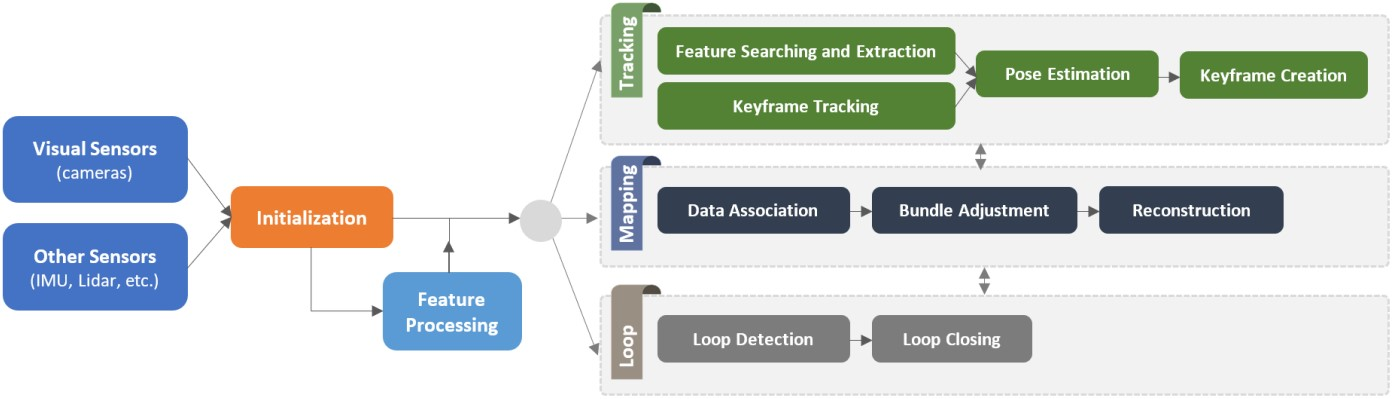
\includegraphics[ width=1\textwidth ]{VSLAM}
    \caption{Funktionsweise des Visual SLAM \cite{tourani2022vSLAMTrends}\label{fig:VSLAM}}\par
\end{figure}

\subsection{Feature Detection}

Die Feature Detection dient der Identifikation von \emph{Feature-Punkten} in Bildern. Dabei handelt es sich um charakteristische Bereiche, die sich durch ihre besondere Struktur oder Helligkeitsverteilung vom restlichen Bild abheben. Zu diesen Bereichen gehören beispielsweise Ecken, Kanten oder markante Texturbereiche. Jeder Feature-Punkt setzt sich aus einem \emph{Key Point}, welcher einem zweidimensionalen Punkt im Bild entspricht, und einem \emph{Deskriptor} zusammen. \cite{gao2021vSLAM, szeliski2022computerVision}

Der Deskriptor entspricht einer numerischen Beschreibung des erkannten Merkmals, um diese über mehrere Bilder hinweg vergleichbar zu machen. Diese Deskriptoren werden in der Regel als Vektoren dargestellt, die die verschiedenen Charakteristiken um den jeweiligen Feature-Punkt erfassen. Übereinstimmende Feature-Punkte werden anhand der Ähnlichkeiten der Deskriptoren im Vektorraum bestimmt. \cite{gao2021vSLAM, szeliski2022computerVision}

Für die Erkennung von Feature-Punkten existieren verschiedene Algorithmen, darunter SIFT (\emph{Scale-Invariant Feature Transform}) \cite{lowe1999sift}, SURF (\emph{Speeded-Up Robust Features}) \cite{bay2006surf} und ORB (\emph{Oriented FAST and Rotated BRIEF}) \cite{rublee2011orb}. Die folgende Tabelle vergleicht die Geschwindigkeit dieser Algorithmen bei der Extraktion von 1000 Feature-Punkten aus demselben Bild \cite{gao2021vSLAM}:

\begin{table}[h]
    \centering
    \begin{tabular}{ccl} 
        \hline
        Algorithmus & Geschwindigkeit (ms) \\ 
        \hline
        SIFT & 5228.7 \\ 
        SURF & 217.3 \\ 
        ORB & 15.3 \\ 
        \hline
    \end{tabular}
    \caption{Vergleich der Geschwindigkeit von Feature-Detection-Algorithmen \cite{gao2021vSLAM}}
    \label{tab:AlgorithmComparison}
\end{table}

Da AR-Anwendungen in Echtzeit arbeiten müssen, spielen neben der Robustheit vor allem die Geschwindigkeit der Algorithmen eine entscheidende Rolle. ORB bietet hierbei einen optimalen Kompromiss zwischen Effizienz und Stabilität und wird daher häufig für AR-Anwendungen verwendet. Daher wird im Folgenden ORB näher erläutert. \cite{gao2021vSLAM, rublee2011orb}

ORB kombiniert zwei bewährte Verfahren: FAST (\emph{Features from Accelerated Segment Test}) zur Erkennung von Feature-Punkten und BRIEF (\emph{Binary Robust Independent Elementary Features}) zur Erstellung kompakter Deskriptoren. \cite{gao2021vSLAM, rublee2011orb}

Der FAST-Algorithmus erkennt Bereiche mit starken Helligkeitskontrasten, indem er benachbarte Pixel um einen zu prüfenden Pixel herum analysiert. Die Abbildung \ref{fig:FAST} zeigt das Prinzip des FAST-Algorithmus. Hierbei wird zunächst ein Pixel \( p \) mit einem Helligkeitswert \( I_p \) ausgewählt. Ausgehend von diesem Pixel werden die Helligkeitswerte der 16 umliegenden Pixel \( p \) auf einer Kreislinie mit einem Radius von 3 Pixel verglichen. Übersteigt die Anzahl der aufeinander folgenden, signifikant helleren oder dunkleren Pixel einen bestimmten Schwellenwert \( N \), wird \( p \) als Feature identifiziert. Diese Schritte werden für alle Pixel im Bild wiederholt, um alle Feature-Punkte zu identifizieren. 

Der Algorithmus kann optimiert werden, indem zunächst die Nachbarpixel 1, 5, 9, und 13 (siehe Abbildung \ref{fig:FAST}) betrachtet werden. Falls drei der vier Pixel heller oder dunkler sind als \( I_p \), kann es sich um einen potenziellen Feature-Punkt handeln. Andernfalls wird der Pixel \( p \) als möglicher Feature-Punkt verworfen. \cite{gao2021vSLAM, rublee2011orb, rosten2006fast}

\begin{figure}
    \centering
    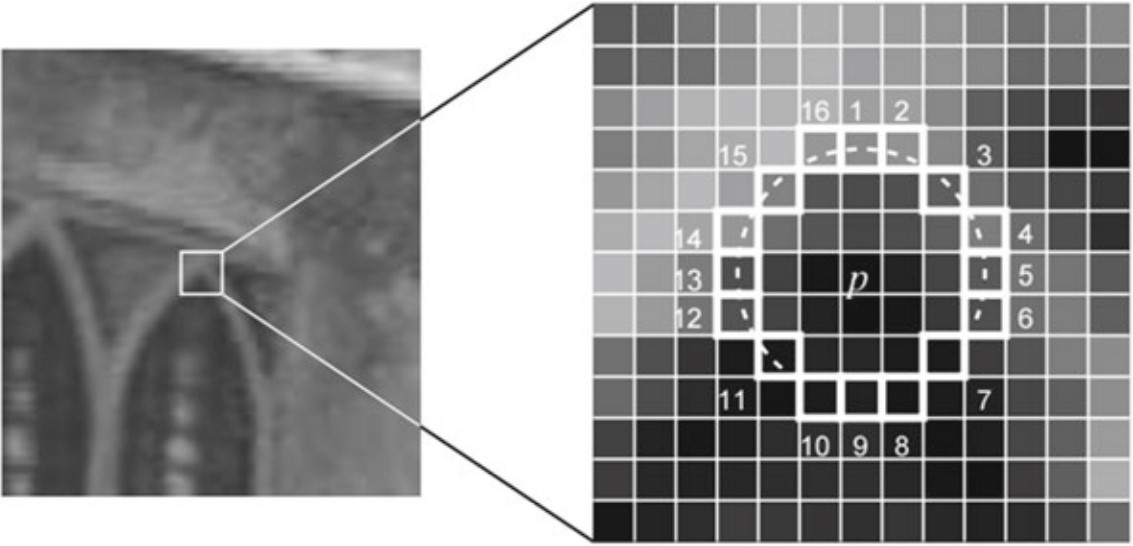
\includegraphics[ width=.5\textwidth ]{FAST}
    \caption{FAST-Feature-Punkte \cite{rosten2006fast}\label{fig:FAST}}\par
\end{figure}

Zusätzlich zu den erkannten Feature-Punkten berechnet ORB Rotations- bzw. Richtungsinformationen für jedes Merkmal. Dazu wird ein sogenannter Zentroid berechnet, der ein Schwerpunkt anhand der Grauwerte des Bildblocks in der Nähe des Feature-Punktes definiert. Diese Zentroide werden wie folgt berechnet \cite{gao2021vSLAM, rublee2011orb}:

Zunächst wird das \emph{Moment} \( m_{pq} \) im Bildblock \( B \) berechnet, wobei \( p \) und \( q \) entweder 0 oder 1 sind:

\begin{equation}
    m_{pq} = \sum_{x,y \in B} x^p y^q I(x, y)
\end{equation}

\begin{tcolorbox}[colback=THAi-Blue!20!white, colframe=THAi-Blue]
    Ein \textbf{Moment} in der Bildverarbeitung ist ein gewichteter Mittelwert der Helligkeitswerte eines Bildes, der bestimmte geometrische oder statistische Eigenschaften wie Fläche, Schwerpunkt oder Ausrichtung beschreibt. \cite{wikipedia2024moment}
\end{tcolorbox}

Mithilfe der Momente kann nun der inhaltsbasierte Schwerpunkt \( C \) (auch ,,centroid'' genannt) des Bildblocks berechnet werden:

\begin{equation}
C = 
\left(
\frac{m_{10}}{m_{00}}, \\
\frac{m_{01}}{m_{00}}
\right)
\end{equation}

Schließlich wird die Orientierung des Features bestimmt, die durch den Vektor \( \overrightarrow{OC} \) vom geometrischen Zentrum des Bildblocks \( O \) zum Zentroiden \( C \) definiert ist und durch den Winkel \( \theta \) beschrieben wird. Die Berechnung kann verkürzt werden, indem der Tangens des Winkels \( \theta \) durch das Verhältnis der Momente \( m_{01} \) und \( m_{10} \) berechnet wird:

\begin{equation}
    \theta = \arctan \left( \frac{m_{01}}{m_{10}} \right)
\end{equation}

Nachdem die Feature-Punkte erkannt wurden, werden die Deskriptoren mithilfe des BRIEF-Algorithmus berechnet. Dazu wird das Bild zunächst mithilfe von Gauß-Filtern geglättet, um Rauschen zu reduzieren. Anschließend erzeugt der BRIEF-Algorithmus binäre Deskriptoren, indem zufällige Pixelpaare um den Feature-Punkt verglichen werden. Ist der Helligkeitswert des ersten Pixels größer als der des zweiten Pixels, wird der binäre Wert 1 gesetzt, andernfalls 0. Die resultierenden binären Werte werden zu einem 128-Bit-Vektor zusammengefügt, der als kompakte und robuste Merkmalsbeschreibung dient. \cite{gao2021vSLAM, calonder2010brief}

Durch die Kombination der FAST-Feature-Detection und der BRIEF-Deskriptoren ermöglicht ORB eine schnelle und robuste Merkmalsextraktion. Die ORB-Features sind invariant gegenüber Rotationen und Skalierungen und eignen sich daher gut für das Feature-Matching. Aus diesem Grund wird ORB häufig in AR-Systemen eingesetzt, um Feature-Punkte zu erkennen und zu beschreiben. \cite{gao2021vSLAM, rublee2011orb}

Neben klassischen Feature-Detection-Verfahren gewinnen Deep-Learning-Modelle zunehmend an Bedeutung für die Feature Detection. Besonders \emph{Convolutional Neural Networks} (CNNs) und Transformer-Modelle liefern vielversprechende Ergebnisse. Ein Beispiel hierfür ist \emph{XFeat} (Accelerated Features), ein optimiertes neuronales Netzwerk, das die Merkmalsextraktion beschleunigt. Auch \emph{OmniGlue}, eine Kombination aus CNNs und Transformer-Modellen, setzt neue Maßstäbe in der robusten und anpassungsfähigen Feature-Matching-Strategie. Diese modernen Ansätze bieten oft eine höhere Genauigkeit und Stabilität, insbesondere in komplexen Szenen oder bei stark variierenden Lichtverhältnissen. \cite{ghosh2024fmNN}

\subsection{Feature Matching}

Das \emph{Feature Matching} ist ein entscheidender Schritt im Visual SLAM, bei dem übereinstimmende Feature-Punkte in aufeinanderfolgenden Bildern identifiziert werden. Diese Übereinstimmungen sind essenziell für die spätere Berechnung der Kamerabewegung. \cite{gao2021vSLAM, szeliski2022computerVision}

Feature-Matching-Algorithmen vergleichen die Deskriptoren der Feature-Punkte und bestimmen deren Ähnlichkeit. Ein naiver Ansatz ist das \emph{Brute-Force-Matching}, bei dem jeder Deskriptor mit allen anderen verglichen wird. Bei BRIEF-Deskriptoren erfolgt dieser Vergleich mithilfe der \emph{Hamming-Distanz}, die angibt, wie viele Bits sich zwischen zwei Deskriptoren unterscheiden. Die Feature-Punkte mit der geringsten Hamming-Distanz werden als übereinstimmende Punkte identifiziert. \cite{gao2021vSLAM, szeliski2022computerVision}

Da die Anzahl der Feature-Punkte in einem Bild hoch sein kann, stößt der Brute-Force-Ansatz schnell an seine Grenzen, insbesondere in Echtzeitanwendungen wie AR-Systemen. Eine effizientere Alternative bietet FLANN (Fast Library for Approximate Nearest Neighbors). FLANN verwendet optimierte Algorithmen, um die Suche nach den nächsten Nachbarn in großen Datensätzen erheblich zu beschleunigen. Dabei kommen unter anderem k-d-Bäume zum Einsatz, die eine strukturierte Partitionierung des Datenraums ermöglichen und so die Berechnung effizienter gestalten. \cite{gao2021vSLAM, muja2009flann}

\subsection{Pose Estimation}

Die Schätzung der Kameraposition (\emph{Pose Estimation}) bildet die Grundlage für die Rekonstruktion der dreidimensionalen Szene. Die Berechnung basiert auf der \emph{Epipolargeometrie}, die die Beziehung zwischen zwei oder mehreren Bildern beschreibt und die Bestimmung der Kameraposition ermöglicht. \cite{gao2021vSLAM} 

Dazu wird die Bewegung der Kamera zwischen den Bildern ermittelt. Diese Bewegung kann mithilfe der \emph{Essential Matrix} dargestellt werden, die die Rotation \( R \) und Translation \( t \) der Kamera zwischen den Bildern definiert. \cite{gao2021vSLAM}

\begin{figure}[h]
    \centering
    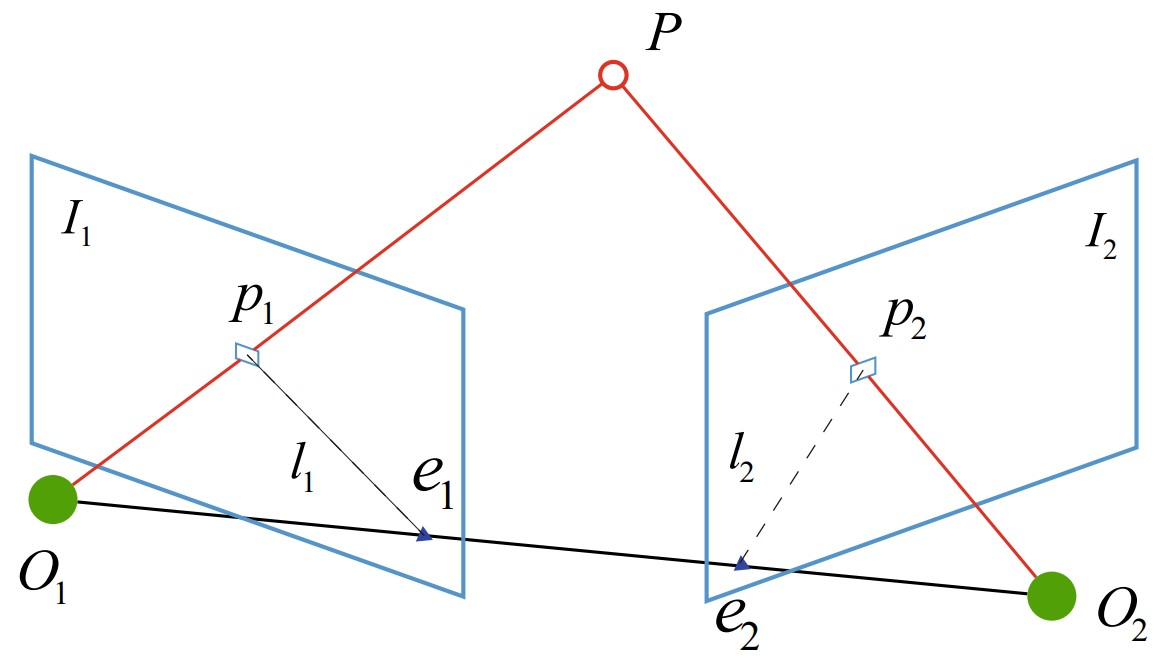
\includegraphics[ width=.5\textwidth ]{Epipolar}
    \caption{Situation der Epipolargeometrie bei zwei Bildern \cite{gao2021vSLAM}\label{fig:Epipolar}}\par
\end{figure}

Betrachten wir die Situation in Abbildung \ref{fig:Epipolar}, in der zwei Bilder \( I_1 \) und \( I_2 \) und die übereinstimmenden Feature-Punkte \( p_1 \) und \( p_2 \) dargestellt sind. Die Kamerapositionen \( O_1 \) und \( O_2 \) sind ebenfalls eingezeichnet. \cite{gao2021vSLAM}

Unter Verwendung des Pinhole-Modells aus Kapitel \ref{Kalibrierung} und der beschriebenen Projektion kann die Bewegung der Kamera zwischen den Bildern wie folgt beschrieben werden \cite{gao2021vSLAM}:
\begin{equation}
    p_1 = KP, \quad p_2 = K(RP + t)
\end{equation}

Dabei entspricht \( R \) der Rotation und \( t \) der Translation der Kamera. Der Punkt \( P \) ist der Schnittpunkt der Linien \( \overrightarrow{O_1p_1} \) und \( \overrightarrow{O_2p_2} \) (siehe Abbildung \ref{fig:Epipolar}). \cite{gao2021vSLAM}

Die epipolare Bedingung besagt, dass die Kamerapositionen \( O_1 \) und \( O_2 \) zusammen mit dem Punkt \( P \) auf einer Ebene liegen. Diese Bedingung kann durch die folgende Gleichung ausgedrückt werden \cite{gao2021vSLAM}:
\begin{equation}
    x_2^T t \times R x_1 = 0\label{eq:Epipolar}
\end{equation}

Hierbei stehen \( x_1 \) und \( x_2 \) für die homogenen Koordinaten der übereinstimmenden Feature-Punkte \( p_1 \) und \( p_2 \) in den Bildern \( I_1 \) und \( I_2 \). Die Essential Matrix \( E \) wird nun wie folgt definiert \cite{gao2021vSLAM}:
\begin{equation}
    E = t \times R
\end{equation}

Diese Matrix entspricht einer 3x3-Matrix mit neun Unbekannten. Geht man nun von \( x_1 = [u_1, v_1, 1]^T \) und \( x_2 = [u_2, v_2, 1]^T \) aus, kann die epipolare Bedingung \ref{eq:Epipolar} in die folgende Gleichung umgeformt werden \cite{gao2021vSLAM}:
\begin{equation}
(u_2, v_2, 1) 
\begin{pmatrix}
    e_1 & e_2 & e_3 \\
    e_4 & e_5 & e_6 \\
    e_7 & e_8 & e_9
\end{pmatrix}
\begin{pmatrix}
    u_1 \\ v_1 \\ 1
\end{pmatrix}
= 0
\end{equation}

Schreiben wir die Matrix \( E \) als Vektor \( e = [e_1, e_2, \ldots, e_9]^T \), können wir die epipolare Bedingung als lineare Gleichung darstellen:
\begin{equation}
    [u_2u_1, u_2v_1, u_2, v_2u_1, v_2v_1, v_2, u_1, v_1, 1] e = 0.
\end{equation}

Die Essential Matrix kann dann mithilfe des \emph{Eight-Point-Algorithmus} geschätzt werden, der die epipolare Bedingung für mindestens acht Punktpaare in den Bildern verwendet. Ein ganzheitliches Gleichungssystem mit allen acht Feature-Punkten kann wie folgt dargestellt werden \cite{gao2021vSLAM, stachniss2020FandEmatrix, hartley1997eightpoint}:
\begin{equation}
    \begin{pmatrix}
        u_2^1 u_1^1 & u_2^1 v_1^1 & u_2^1 & v_2^1 u_1^1 & v_2^1 v_1^1 & v_2^1 & u_1^1 & v_1^1 & 1 \\
        u_2^2 u_1^2 & u_2^2 v_1^2 & u_2^2 & v_2^2 u_1^2 & v_2^2 v_1^2 & v_2^2 & u_1^2 & v_1^2 & 1 \\
        \vdots & \vdots & \vdots & \vdots & \vdots & \vdots & \vdots & \vdots & \vdots \\
        u_2^8 u_1^8 & u_2^8 v_1^8 & u_2^8 & v_2^8 u_1^8 & v_2^8 v_1^8 & v_2^8 & u_1^8 & v_1^8 & 1 
    \end{pmatrix}
    \begin{pmatrix}
        e_1 \\ e_2 \\ e_3 \\ e_4 \\ e_5 \\ e_6 \\ e_7 \\ e_8 \\ e_9
    \end{pmatrix}
    = 0
\end{equation}

Um die Essential Matrix in die Rotationsmatrix \( R \) und den Translationsvektor \( t \) zu zerlegen, wird die \emph{Singulärwertzerlegung} (SVD) verwendet. Die genaue Beschreibung dieser Zerlegung und die Anwendung des Eight-Point-Algorithmus sind keine Bestandteile dieser Arbeit. Stattdessen wird auf weiterführende Literatur verwiesen. \cite{gao2021vSLAM, tsai1984svd, hartley1997eightpoint}

Wichtig ist, dass sich aus der Zerlegung der Essential Matrix vier mögliche Lösungen für \( R \) und \( t \) ergeben, da die Matrix nur die relative Bewegung zwischen zwei Bildern beschreibt. Die Abbildung \ref{fig:SVD} zeigt ein Beispiel für die vier möglichen Lösungen der Zerlegung. Die korrekte Lösung kann durch die Überprüfung der positiven Parallaxe ermittelt werden. Diese gibt an, ob sich die rekonstruierten Punkte vor oder hinter der Kamera befinden. Die richtige Lösung ist diejenige, bei der die meisten Punkte vor der Kamera liegen. \cite{gao2021vSLAM}

\begin{figure}
    \centering
    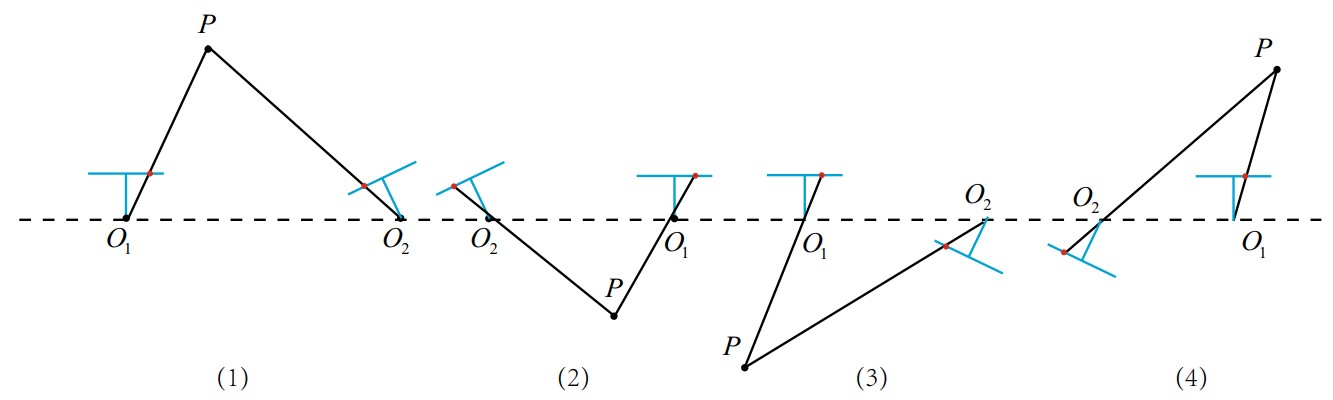
\includegraphics[ width=1\textwidth ]{SVD}
    \caption{Zerlegung der Essential Matrix \cite{gao2021vSLAM}\label{fig:SVD}}\par
\end{figure}

Da die Berechnung der Kamerabewegung nur die relative Pose zwischen zwei Bildern liefert, kann die absolute Position der Kamera nicht direkt bestimmt werden. Um das Weltkoordinatensystem zu definieren, wird in vielen AR-Systemen die Kamera-Position des ersten Bildes als Ursprung des Weltkoordinatensystems festgelegt. Die folgenden Kamerapositionen werden dann relativ zu diesem Ursprung berechnet. \cite{gao2021vSLAM,appledevdoc}

\subsection{Dreidimensionale Rekonstruktion}

Die Rekonstruktion der dreidimensionalen Szene basiert auf der Bestimmung der räumlichen Positionen von Feature-Punkten. Dieser Prozess wird als \emph{Triangulation} bezeichnet und ermöglicht es, aus mehreren Bildern die dreidimensionalen Koordinaten eines Punktes zu berechnen. \cite{gao2021vSLAM}

Abbildung \ref{fig:Triangulation} illustriert das Prinzip der Triangulation eines Punktes \( P \) anhand zweier Bilder. Die Kamerapositionen \( O_1 \) und \( O_2 \) sowie die korrespondierenden Punkte \( p_1 \) und \( p_2 \) sind dargestellt. Der gesuchte Punkt \( P \) entspricht dem gesuchten Feature-Punkt im Raum. In einer idealen Welt entspricht \( P \) dem Schnittpunkt der Geraden \( \overrightarrow{O_1p_1} \) und \( \overrightarrow{O_2p_2} \). Aufgrund von Rauschen und Ungenauigkeiten in den Bildern ist die exakte Bestimmung des Punktes durch die Berechnung des Schnittpunktes meist nicht möglich. Stattdessen kann der gesuchte Punkt durch die Minimierung des quadratischen Abstandes berechnet werden. Der gesuchte Punkt \( P \) ist derjenige, der sich im minimalen Abstand zu allen Strahlen befindet (siehe Abbildung \ref{fig:Triangulation}). \cite{gao2021vSLAM}

\begin{figure}[h]
    \centering
    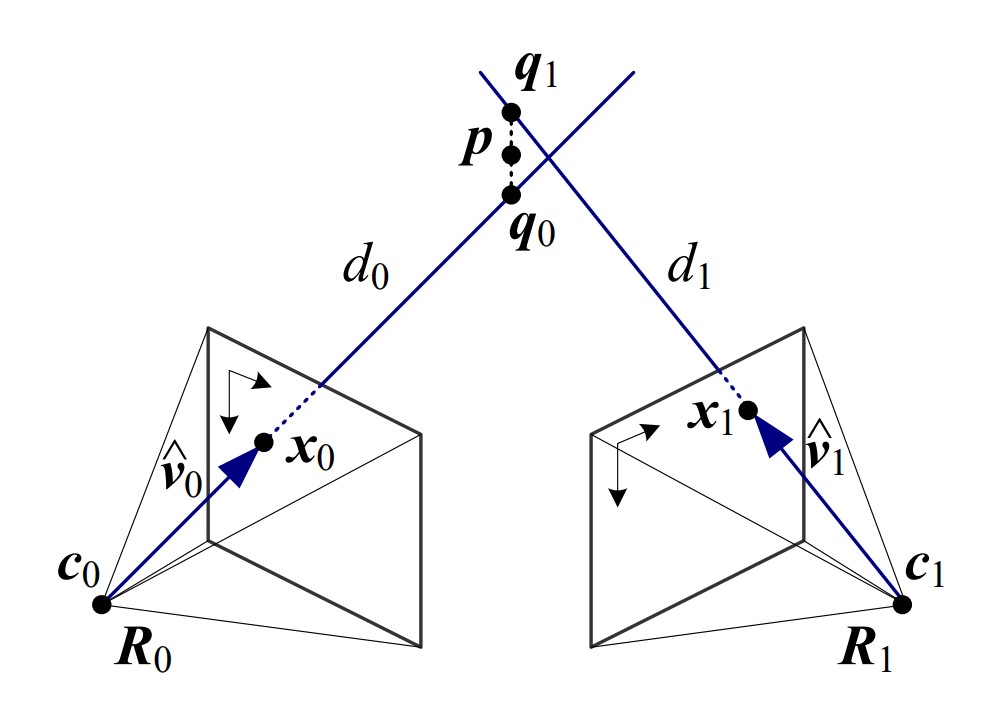
\includegraphics[width=.5\textwidth]{Triangulation}
    \caption{Dreidimensionale Triangulation mit zwei Bildern \cite{gao2021vSLAM}\label{fig:Triangulation}}\par
\end{figure}

Das Ergebnis der Triangulation verschiedener Feature-Punkte über mehrere Bilder ergibt eine sogenannte Punktwolke (\emph{Point Cloud}, siehe Abbildung \ref{fig:PointCloud}), die die 3D-Struktur der Szene abbildet. Diese Punktwolke dient als Grundlage für die weitere Verarbeitung zur Erstellung eines detaillierten 3D-Modells der Szene.

\begin{figure}[h]
    \centering
    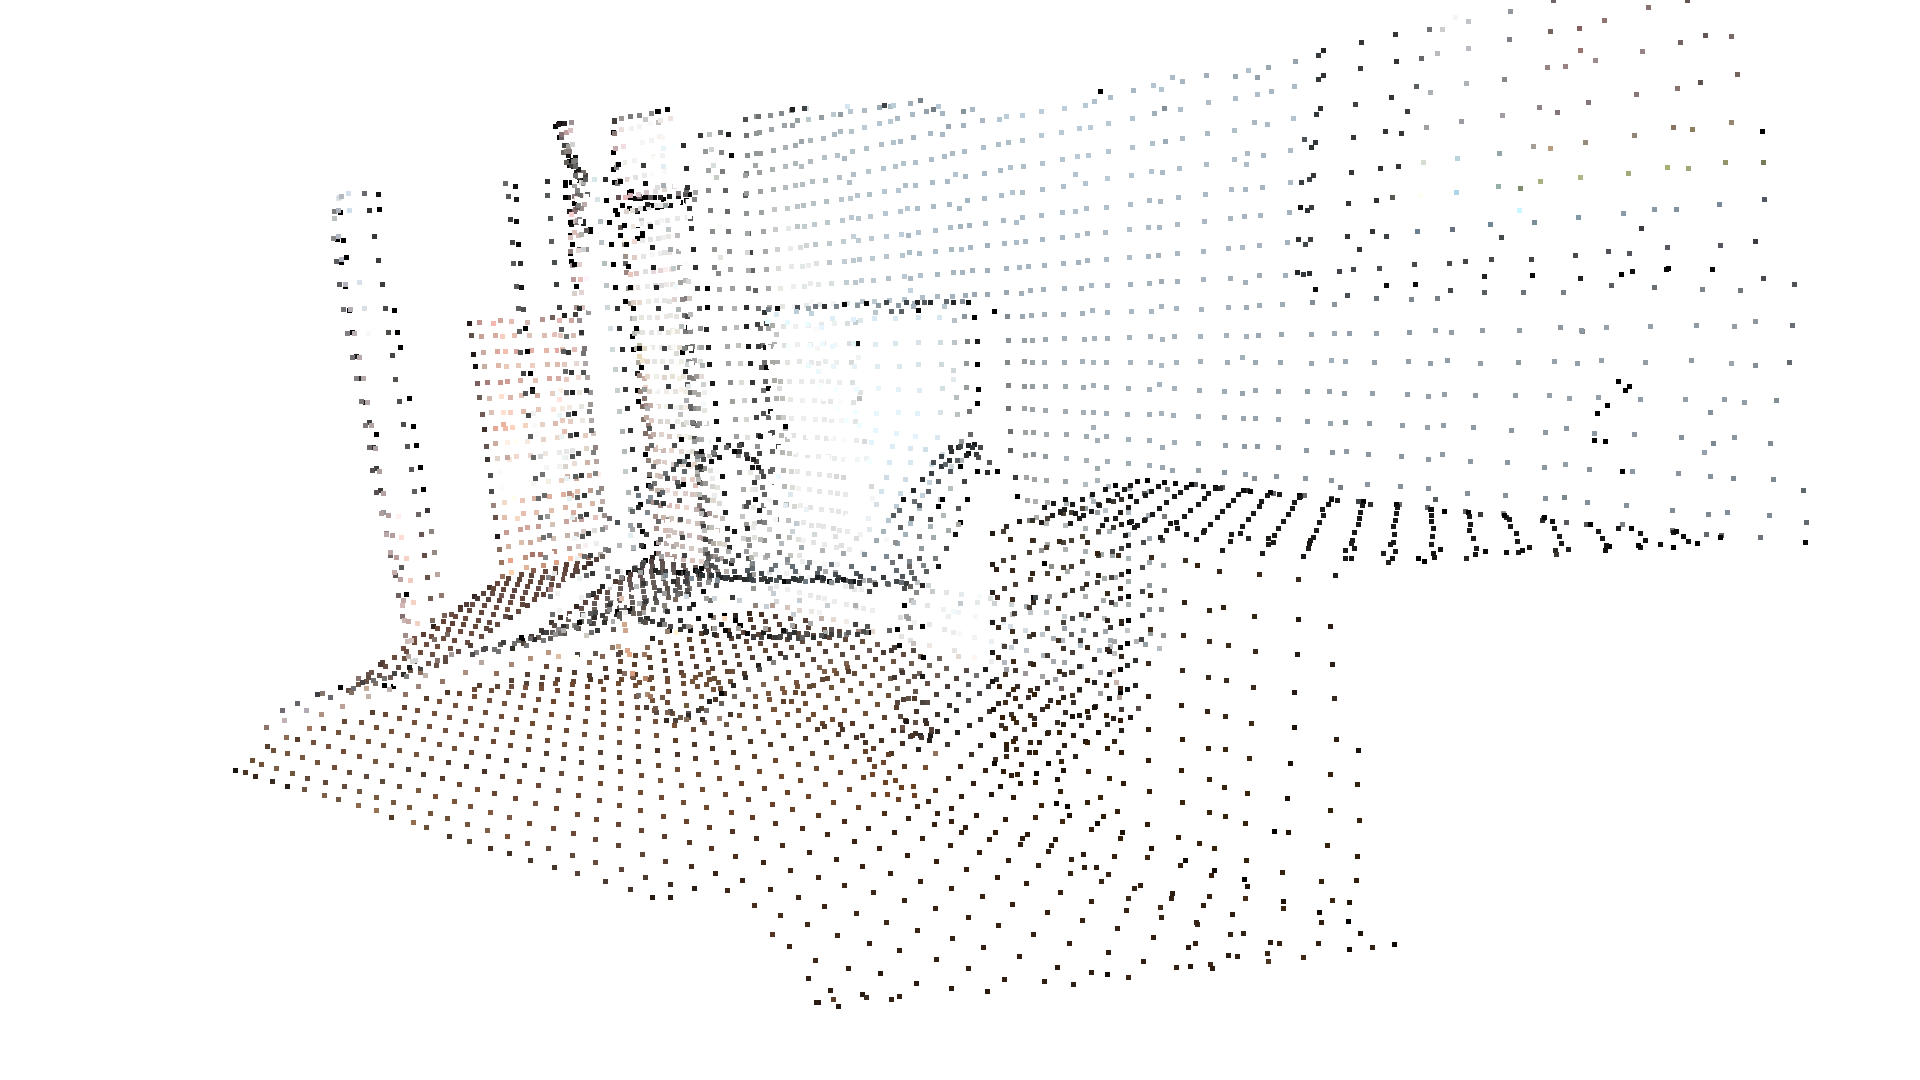
\includegraphics[ width=.5\textwidth ]{PointCloud}
    \caption{Beispiel einer Punktwolke \cite{open3d2025pointcloud}\label{fig:PointCloud}}\par
\end{figure}

Ein gängiges Verfahren zur Weiterverarbeitung ist die \emph{Poisson-Rekonstruktion}. Mithilfe des Algorithmus kann eine glatte, geschlossene 3D-Oberfläche berechnet werden, indem das Problem als Lösung einer \emph{Poisson-Gleichung} formuliert wird. Diese Gleichung entspricht einer elliptischen, partiellen Differentialgleichung, die die Oberfläche der Punktwolke als Lösung approximiert. \cite{kazhdan2006poisson}

Ein weiterer wichtiger Verarbeitungsschritt ist die Erkennung glatter Flächen (\emph{Plane Detection}) in der Punktwolke. Hierbei kommt häufig der RANSAC-Algorithmus (\emph{Random Sample Consensus}) zum Einsatz. Mithilfe dieses Algorithmus können vergleichsweise einfach Flächen segmentiert werden \cite{yang2010planeDetection, ajith2020ransac}:

\begin{enumerate}
    \item Drei zufällige Punkte auswählen, um eine Ebene zu definieren.
    \item Parameter der Ebene berechnen.
    \item Abweichungen der restlichen Punkte von der Ebene mithilfe der Bestimmung der Distanz zwischen den Punkten und der Ebene berechnen.
    \item Falls der Abstand kleiner als ein Schwellenwert ist, den jeweiligen Punkt als zugehörigen Punkt betrachten.
    \item Ebenen mit den meisten zugehörigen Punkten als glatte Flächen betrachten.
    \item Den Prozess bis zu einer bestimmten Anzahl von Iterationen wiederholen.
\end{enumerate}

Durch die Erkennung von Flächen in der Punktwolke können die 3D-Modelle der Szene weiter verfeinert und strukturiert werden. Dies ist insbesondere für die Platzierung virtueller Objekte in der Augmented Reality von Bedeutung. \cite{doerner2022virtual}

\subsection{Bundle Adjustment}

Bei der Rekonstruktion einer Szene treten zwangsläufig Ungenauigkeiten auf. Diese entstehen zum Beispiel durch Bildrauschen, Unsicherheiten bei der Schätzung der Kamerapositionen oder Fehlern bei der Triangulation. Um diese Fehler zu minimieren und eine präzisere Rekonstruktion zu erreichen, wird das \textit{Bundle Adjustment} (BA) eingesetzt. Dieses Verfahren optimiert die gesamte Szene, indem es die Kamerapositionen und die 3D-Feature-Punkte gleichzeitig anpasst. \cite{gao2021vSLAM}

In SLAM-Systemen ist das Bundle Adjustment eine der wichtigsten Methoden zur globalen Optimierung. Ziel ist es, den sogenannten \textit{Reprojektionsfehler} zu minimieren. Dieser Fehler beschreibt die Differenz zwischen den erkannten Feature-Punkten und den reprojizierten Punkten auf der zweidimensionalen Bildebene. Die reprojizierten Punkte können durch die Projektion der triangulierten Feature-Punkte im Weltkoordinatensystem zurück auf die zweidimensionale Bildebene berechnet werden. \cite{gao2021vSLAM}

\begin{figure}
    \centering
    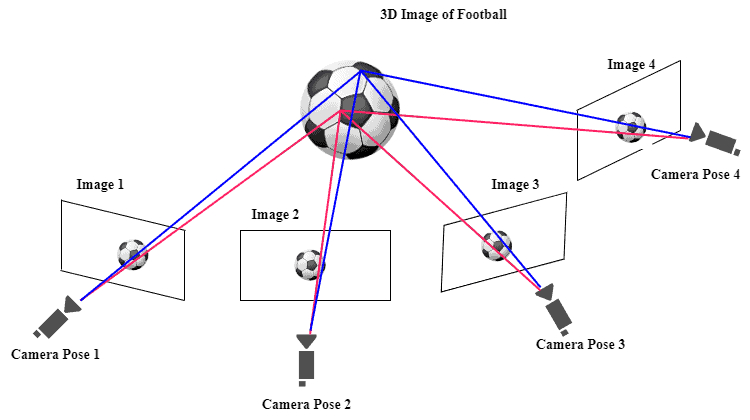
\includegraphics[ width=.8\textwidth ]{BundleAdjustment}
    \caption{Beispiel einer Situation mit Reprojektionsfehler \cite{kumar2024bundleAdjustment}\label{fig:BA}}\par
\end{figure}

Die Abbildung \ref{fig:BA} veranschaulicht den Reprojektionsfehler eines Feature-Punktes. Um diesen triangulierten Punkt zurück in die Bildebene zu projizieren, werden sowohl die extrinsischen als auch die intrinsischen Kameraparameter (siehe Kapitel \ref{Kalibrierung}) benötigt. Die Projektion erfolgt in mehreren Schritten \cite{gao2021vSLAM}:

Zunächst wird der triangulierte Punkt \( P \) unter Berücksichtigung der extrinsischen Kameraparameter \( [R|t] \) in das Bildkoordinatensystem transformiert:
\begin{equation}
    P' = Rp+t = [X', Y', Z']^T
\end{equation}

Anschließend wird der Punkt \( P' \) in die normalisierte Bildebene projiziert:
\begin{equation}
    P_b = [u_b, v_b, 1]^T = \frac{1}{Z'}[X', Y', Z']^T = [X'/Z', Y'/Z', 1]^T
\end{equation}

Unter Verwendung der Verzerrungsmodelle aus Kapitel \ref{Kalibrierung} können die korrigierten Koordinaten \( [u'_c, v'_c] \) des Punktes berechnet werden. Die Anwendung der intrinsischen Parameter liefert die Pixelkoordinaten des reprojizierten Punktes im Bild:
\begin{equation}
    \begin{aligned}
        u_c = Ku'_b = f_xu'_b + c_x \\
        v_c = Kv'_b = f_yv'_b + c_y
    \end{aligned}
\end{equation}

Der Reprojektionsfehler ergibt sich aus der Differenz zwischen dem beobachteten Punkt \( z \) und dem berechneten reprojizierten Punkt \( h(T,p) \):
\begin{equation}
    e = z - h(T,p)
\end{equation}

Somit kann nun eine ganzheitliche Fehlerfunktion formuliert werden, die die Summe der quadrierten Reprojektionsfehler über alle Feature-Punkte und Kamerapositionen darstellt \cite{gao2021vSLAM}:
\begin{equation}
    \frac{1}{2} \sum_{i=1}^{m} \sum_{j=1}^{n} \| e_{ij} \|^2 = \frac{1}{2} \sum_{i=1}^{m} \sum_{j=1}^{n} \| z_{ij} - h(T_i, p_j) \|^2
\end{equation}

Bei dieser Summe handelt es sich um ein nichtlineares Optimierungsproblem, das mithilfe von numerischen Optimierungsmethoden gelöst werden kann. Ein bekanntes Verfahren zur Lösung des Bundle Adjustment ist das Levenberg-Marquardt-Verfahren, das eine Kombination aus dem Gauss-Newton-Verfahren und der Methode der kleinsten Quadrate darstellt. Dieses Verfahren versucht, die Fehlerfunktion iterativ zu minimieren, indem es die Parameter der Kamerapositionen und Feature-Punkte optimiert. \cite{gao2021vSLAM, levenberg2024minimization}

Eine Optimierungsstrategie, die nur die Kameraposenschätzungen betrachtet, ist die sogenannte \emph{Pose Graph Optimization}. Die Abbildung \ref{fig:PoseGraph} verdeutlicht den Unterschied zwischen der Pose Graph Optimization und dem Bundle Adjustment. Während das Bundle Adjustment alle Feature-Punkte und Kamerapositionen in einem einzigen Bündel (,,Bundle'') optimiert, konzentriert sich die Pose Graph Optimization nur auf die Kamerapositionen. Dies ermöglicht eine schnellere und effizientere Optimierung, da die Feature-Punkte oft keine Optimierung benötigen. \cite{gao2021vSLAM}

\begin{figure}
    \centering
    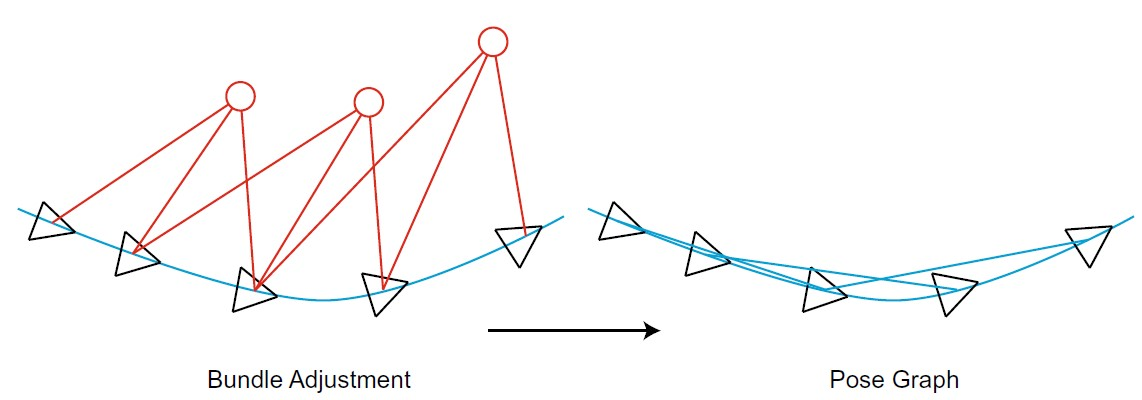
\includegraphics[ width=.8\textwidth ]{PoseGraphOptimization}
    \caption{Bundle Adjustment vs. Pose Graph Optimization \cite{gao2021vSLAM}\label{fig:PoseGraph}}\par
\end{figure}

\subsection{Loop Closure}

Während das Bundle Adjustment die Optimierung von Kamerapositionen und Feature-Punkte über aufeinanderfolgende Bilder hinweg ermöglicht, ist es nicht in der Lage, Fehler zu korrigieren, die durch wiederkehrende Strukturen oder Schleifen in der Szene entstehen. Solche Fehler entstehen durch die Akkumulation von Ungenauigkeiten in den Kamerapositionen und der Feature-Triangulation über längere Sequenzen hinweg. \cite{gao2021vSLAM, cadena2016slam}

Die \textit{Loop Closure Detection} dient dazu, diese Fehler zu erkennen und zu korrigieren. Sie identifiziert bereits besuchte Orte in der Szene und passt die Rekonstruktion der Umgebung sowie die Kamerapositionen entsprechend an. Anstatt einzelne Feature-Deskriptoren direkt zu vergleichen, wird häufig ein globaler Ansatz gewählt, der die Bilder als Ganzes betrachtet und anhand ihrer visuellen Ähnlichkeit bewertet. \cite{gao2021vSLAM, cadena2016slam}

Eine weit verbreitete Methode zur Erkennung von Schleifen ist das \emph{Bag-of-Words}-Modell (BoW). Dabei wird die Ähnlichkeit von Bildern durch sogenannte \emph{visuelle Wörter} beschrieben. Diese Wörter können als Gruppen benachbarter Merkmalspunkte angesehen werden. Ein Wörterbuch mit fixer Größe repräsentiert die häufigsten Wörter in einer Menge an Bildern. Jedes Bild wird dann anhand dieses Wörterbuchs in einen Merkmalsvektor umgewandelt. Ein Bild \( A \) könnte beispielsweise wie folgt kodiert werden \cite{gao2021vSLAM, yoon2024BoW}: 
\begin{equation}
    A = [1, 1, 0]^T
\end{equation}
Hierbei entspricht die Länge des Vektors der Anzahl der Wörter im Wörterbuch. Die Einträge geben an, ob bestimmte visuelle Wörter im Bild vorhanden sind. 

Eine andere Möglichkeit ist die Kodierung der Häufigkeiten der visuellen Wörter in einem Bild \cite{gao2021vSLAM}:
\begin{equation}
    B = [2, 1, 0]^T
\end{equation}
Dieser Vektor \( B \) beschreibt, wie oft die visuellen Wörter \( w_1 \), \( w_2 \), \( w_3 \) in einem Bild vorkommen. 

Die Ähnlichkeit von Bildern kann dann mithilfe von Distanzmaßen, wie dem euklidischen Abstand, wie folgt berechnet werden \cite{gao2021vSLAM}:
\begin{equation}
    s(\mathbf{A}, \mathbf{B}) = \|\mathbf{A} - \mathbf{B}\|
\end{equation}

Wobei \( A \) und \( B \) die Merkmalsvektoren der Bilder sind. Die Distanz \( s \) kann als Maß für die Ähnlichkeit (\emph{Score}) der Bilder interpretiert werden. Ein Score von 0 bedeutet, dass die Bilder identisch sind, während ein hoher Score auf eine geringe Ähnlichkeit hinweist. Abhängig von einem Schwellenwert können somit mögliche Schleifen in der Szene erkannt werden. \cite{gao2021vSLAM}

Um das visuelle Wörterbuch zu erstellen, werden die Merkmalspunkte der Bilder mithilfe des k-Means-Algorithmus in Cluster unterteilt und in einem k-d-Baum (siehe Abbildung \ref{fig:Dictionary}) organisiert. Diese Unterteilung wird so lange wiederholt, bis die gewünschte Tiefe des Baumes erreicht ist. Die Blätter des Baumes entsprechen den visuellen Wörtern im Wörterbuch. \cite{gao2021vSLAM}

Der k-Mean-Algorithmus ist ein Verfahren, das die Merkmalspunkte in \( k \) Cluster unterteilt. Es funktioniert wie folgt \cite{teynor2024ml}:

\begin{enumerate}
    \item Initialisierung von k zufälligen Clusterzentren.
    \item Zuweisung jedes Punktes zum nächstgelegenen Clusterzentrum.
    \item Neuberechnung der Clusterzentren als Mittelwerte der zugehörigen Punkte.
    \item Wiederholung der Schritte 2 und 3, bis die Clusterzentren konvergieren.
\end{enumerate}

\begin{figure}[h]
    \centering
    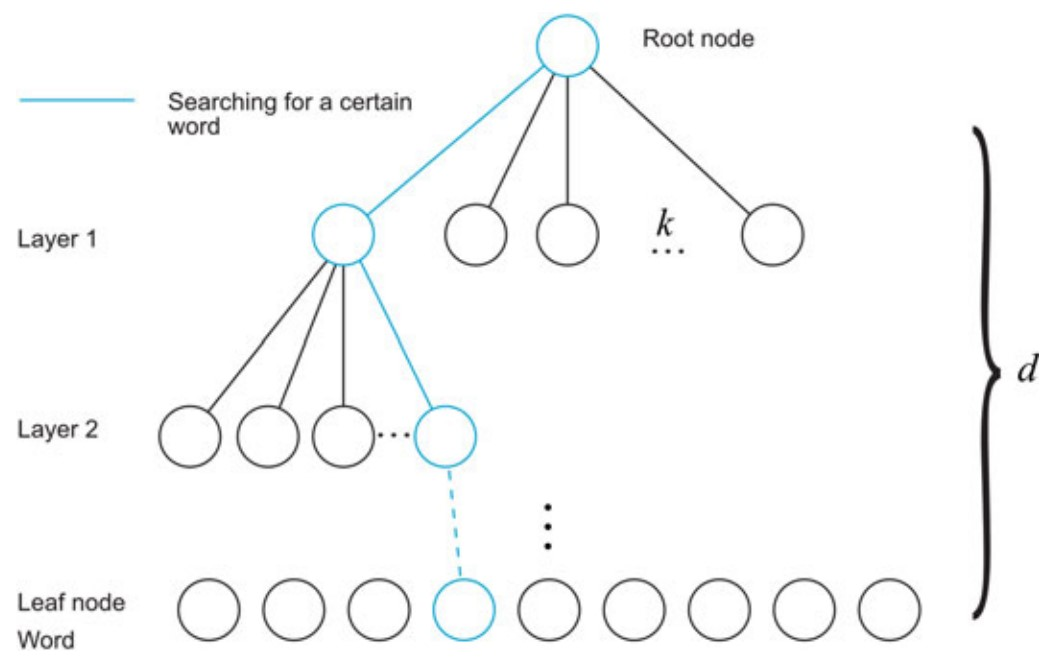
\includegraphics[ width=.5\textwidth ]{Dictionary}
    \caption{Aufbau eines Wörterbuchs mithilfe eines k-d-Baumes \cite{gao2021vSLAM}\label{fig:Dictionary}}\par
\end{figure}

\begin{tcolorbox}[colback=THAi-Blue!20!white, colframe=THAi-Blue]
    \textbf{Clustering} ist ein Algorithmus des unüberwachten, maschinellen Lernens, bei dem ähnliche Objekte in Gruppen (Cluster) zusammengefasst werden. Ziel ist es, Muster oder Strukturen in unklassifizierten Daten zu erkennen. \cite{wikipedia2025clusteranalyse}
\end{tcolorbox}

Das Wörterbuch kann entweder im Vorfeld mithilfe von großen Datensätzen trainiert werden oder während des SLAM-Prozesses inkrementell aufgebaut werden. \cite{ta2023loopClosure, khan2015ibuild, gao2021vSLAM}

\section{Scene Understanding} \label{sec:SceneUnderstanding}

Scene Understanding bezeichnet die Fähigkeit eines Systems, die Umgebung zu interpretieren und zu verstehen. Es existiert eine Vielzahl von Techniken und Methoden, um die Szene zu analysieren. Dazu zählen zum Beispiel die Objekterkennung, die Gesichtserkennung oder die \emph{semantische Segmentierung}. \cite{szeliski2022computerVision}

Die semantische Segmentierung ermöglicht es, die Pixel eines Bildes in verschiedene Klassen, wie beispielsweise Wände, Decken oder Möbel, zu unterteilen. Dadurch lassen sich einzelne Elemente der Szene identifizieren und voneinander unterscheiden. Besonders in der Augmented Reality spielt die semantische Segmentierung eine entscheidende Rolle, da sie die Grundlage für die Interaktion zwischen virtuellen und realen Objekten bildet. \cite{szeliski2022computerVision, appledevdoc, arcoredevdoc}

Frühere Verfahren zur semantischen Segmentierung basierten auf klassischen Bildverarbeitungstechniken wie der histogrammbasierten oder der regionenbasierten Segmentierung. Diese Methoden analysieren Farbverteilungen oder Gruppierungen von benachbarten Pixeln mit ähnlichen Eigenschaften, um verschiedene Bereiche im Bild zu identifizieren. Allerdings stoßen diese Techniken an ihre Grenzen, insbesondere bei der Erkennung komplexer Strukturen oder der Unterscheidung visuell ähnlicher Objekte. \cite{szeliski2022computerVision}

In den letzten Jahren haben sich Deep-Learning-Modelle, insbesondere Convolutional Neural Networks (CNNs), als effektive Methode für die semantische Segmentierung etabliert. Ein bekanntes CNN-Modell für die semantische Segmentierung ist die Fully-Convolutional-Neural-Network-Architektur (FCNN), die speziell für die Segmentierung von Bildern entwickelt wurde. FCNNs sind in der Lage, komplexe Muster in den Bildern zu erkennen und die Pixel in verschiedene Klassen zu segmentieren. \cite{long2014fcnn}

Die FCNN-Architektur besteht aus mehreren Convolutional-Schichten (siehe Abbildung \ref{fig:FCNN}), die die Klassifizierung pro Pixel implementieren. Auf eine detaillierte Beschreibung der Funktionsweise von FCNNs wird aufgrund des gesetzten Rahmens dieser Arbeit verzichtet. Stattdessen wird auf weiterführende Literatur verwiesen. \cite{long2014fcnn, ronneberger2015unet}

\begin{figure}
    \centering
    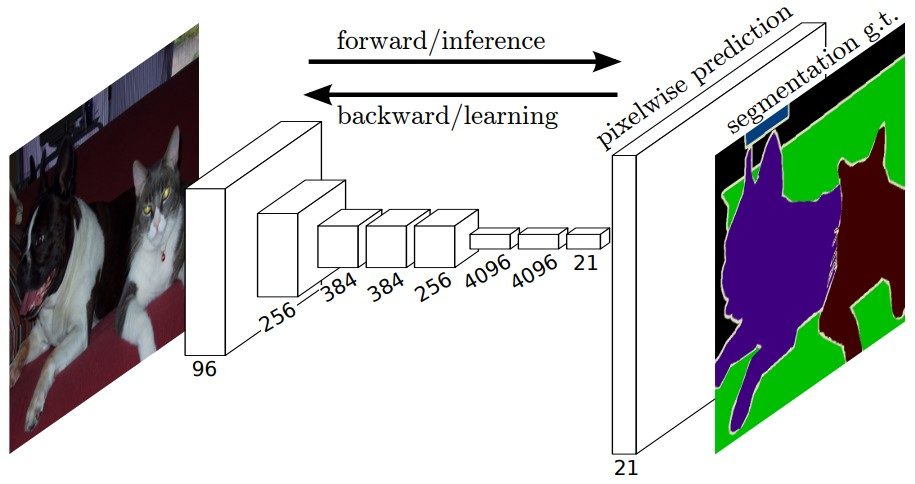
\includegraphics[ width=.5\textwidth ]{FCNN}
    \caption{Darstellung der FCNN-Architektur \cite{long2014fcnn}\label{fig:FCNN}}\par
\end{figure}

\section{LiDAR-Inertial-Visual (LIV) Fusion} \label{sec:LIV}

Einige Augmented Reality Frameworks ermöglichen die Verwendung von LiDAR-Sensoren, sofern die entsprechenden mobilen Geräte mit dieser Art von Sensor ausgestattet sind. Wie in Kapitel \ref{LiDAR} erfassen diese Sensoren mithilfe von Lasern präzise dreidimensionale Punktwolken der Umgebung. \cite{appledevdoc, doerner2022virtual}

Da ein reines LiDAR-SLAM-System keine visuellen Informationen der Kamera nutzt um die Szene zu interpretieren, wird häufig eine Fusion von LiDAR- und Kameradaten vorgenommen. Zusätzlich können IMU-Daten verwendet werden, um die Bewegung des Geräts zu schätzen. Die Kombination dieser drei Sensoren wird als \emph{LiDAR-Inertial-Visual (LIV) Fusion} bezeichnet. \cite{zhang2024lidarslam}

Faktisch ergänzen sich die verschiedenen Sensoren in ihren Stärken und Schwächen. Während LiDAR-Sensoren präzise Distanzinformationen liefern, sind sie anfällig für Rauschen und haben Schwierigkeiten bei der Erfassung von Texturen oder Farben. Kamera-Sensoren hingegen liefern detaillierte visuelle Informationen, sind jedoch anfällig für schlechte Lichtverhältnisse oder schnelle Bewegungen. IMU-Sensoren können die Bewegung des Gerätes schätzen, sind jedoch anfällig für Driftfehler. Somit wird eine weitaus präzisere und robustere Rekonstruktion der Szene als beim reinen vSLAM beziehungsweise LiDAR-SLAM ermöglicht. \cite{zhang2024lidarslam}

Die Integration von LiDAR-, Kamera- und IMU-Daten kann auf zwei Arten erfolgen \cite{zhang2024lidarslam}:
\begin{itemize}
    \item \textbf{Loosely Coupled Fusion:} Hier werden die Sensordaten unabhängig voneinander verarbeitet und erst im Nachhinein fusioniert. Dies ermöglicht eine einfachere Implementierung, kann jedoch zu geringerer Präzision führen, da die Sensoren nicht direkt in einem gemeinsamen Modell optimiert werden.
    \item \textbf{Tightly Coupled Fusion:} Bei diesem Verfahren werden alle Sensordaten innerhalb eines einzigen Optimierungsprozesses verarbeitet. Dadurch lassen sich genauere Schätzungen der Kameraposition und der dreidimensionalen Rekonstruktion erzielen. Allerdings ist dieser Ansatz rechenaufwändiger und komplexer zu implementieren.
\end{itemize}

\begin{figure}
    \centering
    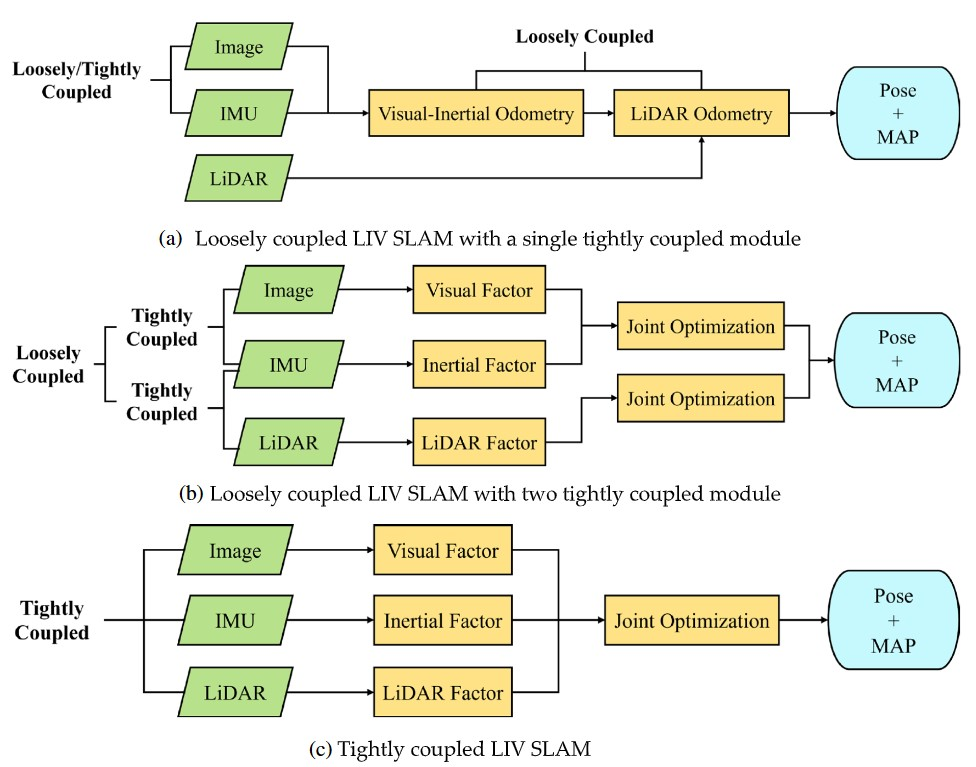
\includegraphics[ width=.8\textwidth ]{LIVSLAM}
    \caption{Mögliche LIV-SLAM-Architektur \cite{zhang2024lidarslam}\label{fig:LIVSLAM}}\par
\end{figure}

Die Abbildung \ref{fig:LIVSLAM} zeigt eine lose gekoppelte Architektur. Dabei werden die Daten der verschiedenen Sensoren zunächst unabhängig voneinander verarbeitet. Die visuell-inertiale Odometrie (VIO) kombiniert die Bilddaten mit den IMU-Daten, um die Bewegung des Gerätes zu schätzen. Die LiDAR-Odometrie (LIO) hingegen schätzt die Bewegung des Gerätes anhand der LiDAR-Daten. Die beiden Schätzungen werden anschließend fusioniert, um eine präzisere und robustere Schätzung der Kameraposition zu erhalten. \cite{zhang2024lidarslam}

Die LiDAR-Odometrie unterscheidet sich von der visuellen Odometrie, da keine Extraktion von Feature-Punkten erforderlich ist. Stattdessen wird die Bewegung des Geräts direkt aus den LiDAR-Daten abgeleitet. Ein gängiger Algorithmus zur Schätzung der Bewegung zwischen zwei LiDAR-Punktwolken ist der \emph{Iterative Closest Point} (ICP) Algorithmus. Die Abbildung \ref{fig:ICP} zeigt wie der ICP-Algorithmus funktioniert. Die zwei Punktwolken ,,rot'' und ,,blau'' werden so transformiert, dass sie möglichst aufeinander liegen. Die Transformation wird iterativ berechnet, bis die Punktwolken übereinstimmen. Daraus kann die Bewegung der Kamera abgeleitet werden. Der ICP-Algorithmus funktioniert wie folgt \cite{gao2021vSLAM, bogoslavskyi2017icp}:

\begin{enumerate}
    \item Initialisierung der Kameraposition.
    \item Berechnung des nächsten Nachbarn für jeden Punkt der blauen Punktwolke in der roten Punktwolke.
    \item Schätzung der Transformation, die die blaue Punktwolke an die rote Punktwolke anpasst.
    \item Anwendung der Transformation auf die blaue Punktwolke.
    \item Wiederholung der Schritte 2 bis 4, bis die Transformation konvergiert.
\end{enumerate}

\begin{figure}[h]
    \centering
    \begin{minipage}{0.24\textwidth}
        \centering
        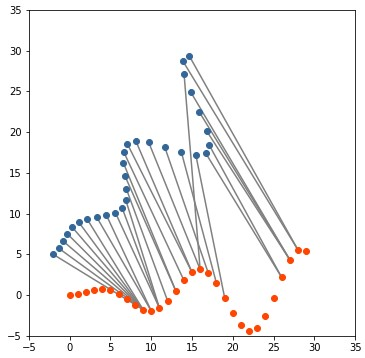
\includegraphics[width=\textwidth]{ICP1}
    \end{minipage}
    \hfill
    \begin{minipage}{0.24\textwidth}
        \centering
        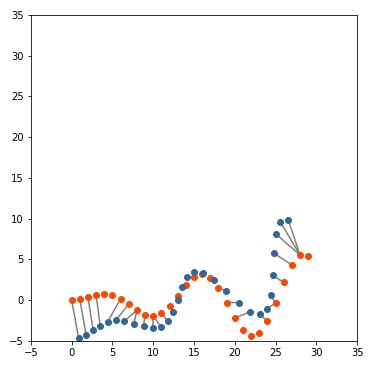
\includegraphics[width=\textwidth]{ICP2}
    \end{minipage}
    \hfill
    \begin{minipage}{0.24\textwidth}
        \centering
        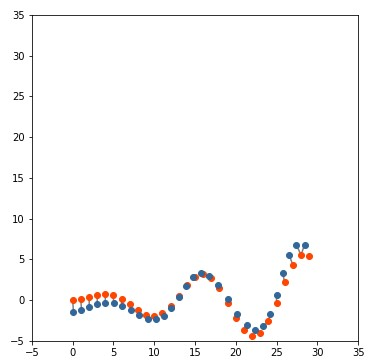
\includegraphics[width=\textwidth]{ICP3}
    \end{minipage}
    \hfill
    \begin{minipage}{0.24\textwidth}
        \centering
        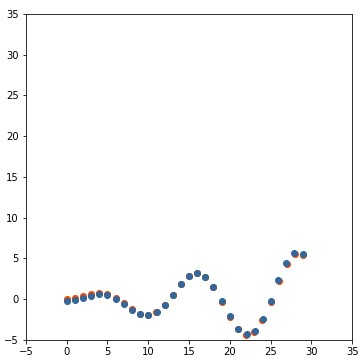
\includegraphics[width=\textwidth]{ICP4}
    \end{minipage}
    \caption{Darstellung des ICP-Algorithmus \cite{bogoslavskyi2017icp}}
    \label{fig:ICP}
\end{figure}

Die Implementierung dieser LIV-Architektur unter Verwendung des ICP-Algorithmus ermöglicht eine einfache und effiziente Lösung für die LIV-Fusion, jedoch ohne eine vollständige, gemeinsame Optimierung aller Sensordaten zu integrieren. \cite{zhang2024lidarslam}